
#### {Adding lines}



\section*{Adding Lines to a Scatter Plot}
Previously we have used scatter plots to plot bivariate data. They were constructed using the \texttt{\textbf{plot()}} command.  

Using the \texttt{\textbf{abline()}} command, we can add lines to our scatter plots. We specify the argument according to the type of line required. A demonstration of three types of line is provided below.



<pre>
<code>

plot(mtcars$mpg,mtcars$wt,pch=18,col="red")
title("Cars Data Set",sub="MPG v Weight")

# Now to Add Lines
abline(v=mean(mtcars$mpg))
abline(h=mean(mtcars$wt))
abline(a=5,b=-1/6)
</code>
</pre>

% \begin{center}[h!]
~% 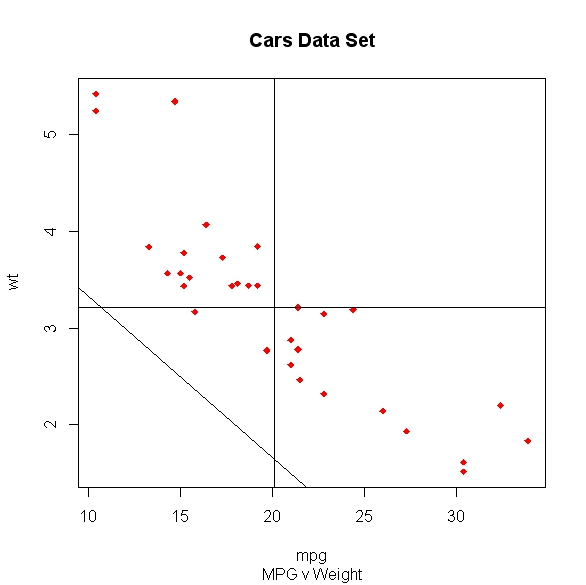
\includegraphics[scale=0.55]{linesDemo}
% \end{center}

Additionally we change the colour of the added lines, by specifying a colour in the \texttt{\textbf{col=}} argument. Finally we can change the line type to one of four possible types, using the lty argument.
The line types are follows 

* \texttt{\textbf{lty =1}}   Normal full line (default)
* \texttt{\textbf{lty =2}}  Dashed line 
* \texttt{\textbf{lty =3}}   Dotted line
* \texttt{\textbf{lty =4}}   Dash-dot line



#### {Adding lines}

Recall that we can use the arguments \texttt{xlim} and \texttt{ylim} to control the vertical and horizontal range of the plots, by specifying a two element vector (min and max) for each.

Using the \texttt{abline()} command, we can add lines to our scatter plots. We specify the argument according to the type of line required. A demonstration of three types of line is provided below.

Additionally we change the colour of the added lines, by specifying a colour in the \texttt{col} argument. We can also change the line type to one of four possible types, using the \texttt{lty} argument.

%=====================================================================================================================%

<pre> 
<code>
x<-rnorm(10)
y<-rnorm(10)
plot(x,y)
plot(x,y,xlim=c(-4,4),ylim=c(-4,4))

# add a vertical dotted line (here the y-axis) to the plot
abline(v =0 , lty =2 ) 

# add a horizontal dotted line (here the x-axis) to the plot
abline(h=0  ,lty =3)    

# add a line to your plot with intercept "a" and slope "b"
abline(a=0,b=1,col="green") 
</code>
</pre>
 
\subsubsection{Adding a Regresion Line to a Plot}
In regression models, scatterplots are often used to depict the relationship between the predictor variable ($x$) and a response variable ($y$).


<pre>
<code>
Fit1 = lm(mpg~wt,data=mtcars)
coef(Fit1)

#(Intercept)          wt 
#  37.285126   -5.344472 

plot(wt,mpg,pch=18,col="red")
abline(coef(Fit1))
</code>
</pre>
%\begin{center}
%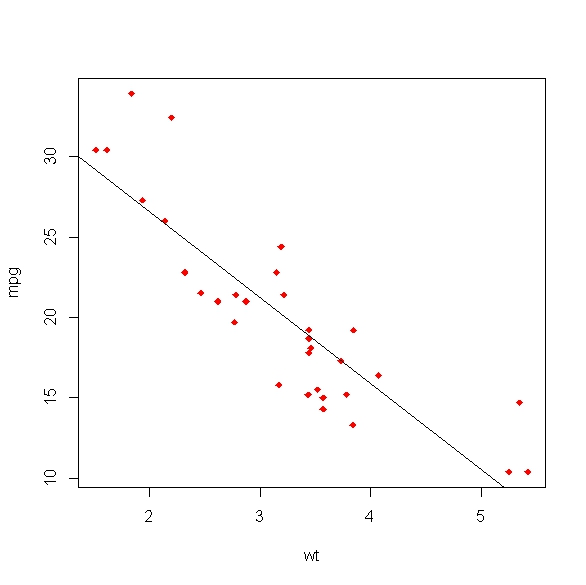
\includegraphics[scale=0.35]{coefPlot}
%\end{center}
\[IMAGE\]
%#### {Line Types and Line Width}
%To specify a line width, we use the \texttt\textbf{{lwd=}} argument.


#### *{\texttt{abline()}}

Using the \texttt{abline()} command, we can add lines to our scatter plots. We specify the argument according to the type of line required. A demonstration of three types of line is provided below.
Additionally we change the colour of the added lines, by specifying a colour in the \texttt{col} argument. We can also change the line type to one of four possible types, using the \texttt{lty} argument.


The line types are follows

	\item	\texttt{lty =1}   Normal full line (default)
	\item	\texttt{lty =2}   Dashed line
	\item	\texttt{lty =3}   Dotted line
	\item	\texttt{lty =4}   Dash-dot line

\footnotesize 






#### {Adding the regression model line}

The \texttt{abline()} function can be used to add a regression model line  by supplying as an argument the \texttt{coef()} values for intercept and slope estimates .These estimates can be inputted directly by using both functions in conjunction.

\footnotesize <code>
Fit1 =lm(y1~x);  coef(Fit1)
abline(coef(Fit1))	
</code>

\end{document}
